\chapter{Background}

\section{Acoustic data}
    This section will explain the basics behind acoustic data, and how it has similar properties to image data. This important to understanding in relation to the machine learning techniques explained later in this chapter. 
    
    Echo sounders are a maritime instrument which induces acoustic waves into the water and logs the backscattered soundwaves\cite{brautaset2020acoustic}. A single emission is called a ping, and is stored is stored as values. In acoustic trawl missions, the multi-frequency echo sounders are mounted on ships and pings on all frequencies chosen for the mission at the same time, with a set interval, and records while traversing an area of interest. As a result, you create what is called an \textit{echogram} which is the representation of the backscattered acoustic waves' encoded as  per frequency. Range is equivalent to \textit{depth}. The frequencies in an echogram can be viewed as the color channels in a picture, each a different representation of the same context. Hence, enabling machine learning techniques to be applied to \textit{echograms}. Below is an example:
    
    
    \begin{figure}[H]
        \centering
        
        \subfloat[Frequency channels that form an echogram. This example show the \gls{sv} per pixel, on the log scale.]{
        	\includesvg[inkscapelatex=false,width=0.4\textwidth,keepaspectratio]{figures/freq_stacked.svg}}
        	%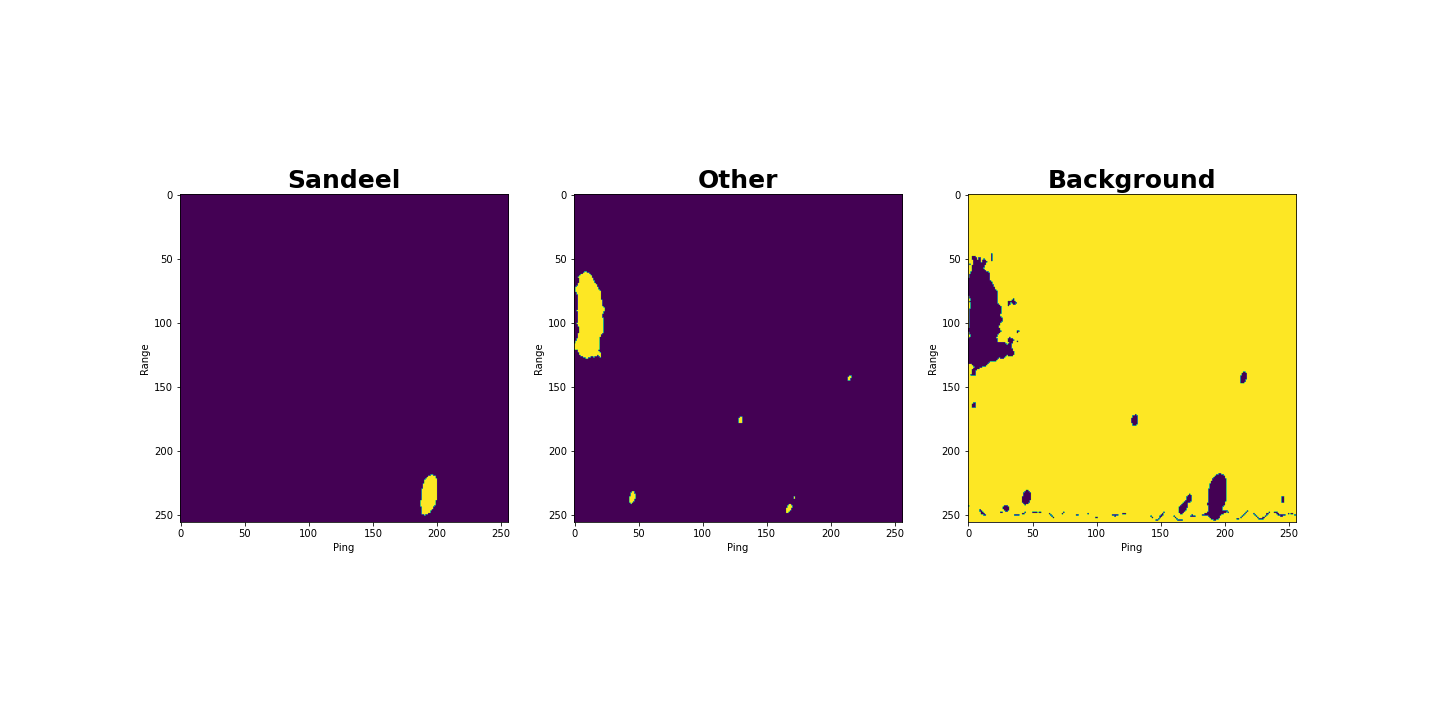
\includegraphics[width=1\textwidth]{figures/data_sample.png} } 
        
        \subfloat[Color channels RGB that forms a picture.]{
        	\includesvg[inkscapelatex=false,width=0.9\textwidth,keepaspectratio]{figures/colors_and_OG.svg}}
        
        
        \caption[Frequency channels and color channels]{How data from echo sounders relate to image data.}
        \label{accoustic data and color channels fig}
        
        \end{figure}
    
    
    
    
    
\section{Machine Learning} \label{Machine Learning}
    As described in the book Deep Learning\cite{Goodfellow-et-al-2016_ML} machine learning can intuitively be split into four parts; The algorithm, empirical data, a task and a performance measure. A machine learning algorithm can then be identified as an algorithm that increases its performance on a task, given data. As this happens, the algorithm is said to be learning. The task itself and the data the algorithm is given may vary. This is why we can approximately divide the machine learning approaches into three categories\cite{Goodfellow-et-al-2016_E}: supervised learning, unsupervised and reinforcement learning. 
    
    \subsection{Algorithm types} \label{Algorithm types}
        \subsubsection{Supervised learning}
            Supervised learning \cite{Goodfellow-et-al-2016_E} algorithms base themselves on datasets containing samples that also have a label. This means the output the algorithm will have to predict. These labels can for example be binary class or consist of a multitude of classes or values in regression problems.
            
        \subsubsection{Unsupervised learning}
            Unlike supervised leaning, the unsupervised learning \cite{Goodfellow-et-al-2016_E} algorithms only have the data and will learn properties contained in the data. A practical example is clustering, where you can divide a dataset into clusters based on similar features. 
                
        \subsubsection{Reinforcement learning}
            In reinforcement learning \cite{Goodfellow-et-al-2016_E}, the algorithm do not learn from a given dataset, but will act in an environment. In some cases this is a feedback loop giving either a positive or negative reward for performing certain actions. The goal is then for the algorithm to maximize this reward. This is what people often associate with \gls{ai} and can be for example seen in the AlphaZero software that beat professional chess players\cite{silver2017mastering}.
    
    \subsection{Data}
        things
    \subsection{Features}
        things
    \subsection{Overfitting vs. underfitting}
        things
    \subsection{Bias - variance tradeoff}
        things
        
    \subsection{Model evaluation}
        In this section, I will describe the tools used to measure my models performances. This can be used to select the best model from a list of models, or gain more insight into the behavior of each or discover errors in the training process.
    \subsubsection{Train-Validation-Test split}
        The goal, when a machine learning model is learning, is to achieve the lowest \textit{generalization error} \cite{Goodfellow-et-al-2016_generalization}. This means to not only perform well on data from the current dataset, but also on a new dataset. To measure this, it is normal to split your data into three parts\cite{Goodfellow-et-al-2016_train_val_test_split}. First the \textit{training} dataset, which will be used in various ways to achieve a low \textit{training error} and is used during learning. The next part, called the \textit{validation} dataset, is drawn from the training dataset and performance on this is an estimate of the generalization error and have many utilities that will be explained later in this thesis. The final and third part is called the \textit{test} dataset and are not touched throughout the training process. It is on this test dataset that the true \textit{generalization error} of a model is calculated. 
    \subsubsection{F1-score, Precision, Recall} \label{f1_score}
        To explain the measurement of a classification model's performance, I will do it by looking into a binary classification system that classifies samples into either the \textit{positive} or \textit{negative} class\cite{powers2020evaluation_f1_recall_precision}. The predictions from this system can then be sorted as follows:
        
        \begin{itemize}
            \item \textbf{True positive (TP):} A correct classification of a positive example.
            \item \textbf{True negative (TN):} A correct classification of a negative example.
            \item \textbf{False positive (FP):} Predicted the positive class, but it was actually negative.
            \item \textbf{False negative (FN):} Predicted the negative class, but it was actually positive.
            \end{itemize}
        
        We can now calculate a performance from these values, and the simplest is accuracy\cite{powers2020evaluation_f1_recall_precision}:
        
        \begin{equation}
            accuracy = \dfrac{TP+TN}{TP+TN+FP+FN} 
        \end{equation}
        
        This metrics weakness is that is does not handle class imbalance well\cite{powers2020evaluation_f1_recall_precision}, as it is equivalent to calculating the percentage of correct predictions. The example being that if 95\% of the data belongs to one class, then always predicting this class will give you an accuracy of 95\%.
        
        To deal with the class imbalance issue, you calculate two new metrics\cite{powers2020evaluation_f1_recall_precision}. First \textit{precision}, which is the percentage of positive predictions made by the model that are actually correct. Secondly, \textit{recall}, which is the percentage of all positive samples the model managed to classify correctly. The formulas are shown below:
        
        \begin{equation}
            \textrm{precision} = \dfrac{TP}{TP+FP}
        \end{equation}
        
        \begin{equation}
            \textrm{recall} = \dfrac{TP}{TP+FN}
        \end{equation}
        
        Then, by using precision and recall, you calculate the \textit{F1-score}, which is the harmonic mean between them\cite{powers2020evaluation_f1_recall_precision}. It combines these metrics and is designed to work well on imbalanced data. There are other metrics that could be calculated, but those mentioned in this section are the ones used in this work. The F1-score formula:
        
        \begin{equation}
            \textrm{F1-score} = 2 * \dfrac{\textrm{precision} * \textrm{recall}}{\textrm{precision} + \textrm{recall}}
        \end{equation}
        
        
        \todo{etter beskivelse av over-underfit, knytt hvordan du kan lese av convergence og andre problemer via train-val-test observasjon}


\section{Artificial Neural Networks} \label{neural networks}
    In this section, I will introduce the basic components of an \gls{ann} and how these are combined to create a complete network.

    \subsection{Perceptron} \label{perceptron}
        The \gls{ann}s fundamental building block is called an artificial \textit{neuron} or perceptron. It is formulated in the following way\cite{razavi2021deep_exp_per}:
            \begin{equation} \label{eq_perceptron}
                y = \sigma(\sum_{i=1}^{D}w_ix_i + b)
            \end{equation}
            
        where D is the number dimension of the input space, x is the input vector and w is a set of weights that is of the same size as x, b is the bias and {\textsigma} is a nonlinear activation function which will be explained later in \ref{activation function}. In short, the equation inside the activation functions is a linear regression with the tunable parameters w and b. The perceptron is illustrated in figure \ref{Perceptron / MLP}.
    
    \subsection{Multi-layered perceptron} \label{MLP}
        The neurons presented in section \ref{perceptron} are then copied and sorted together in layers to form a \gls{ann}, which in turn forms what is called a \gls{mlp} \cite{razavi2021deep_exp_per}. All the neurons in each layer are connected to every neuron in the next layer, as depicted in figure \ref{Perceptron / MLP}.
        
            \begin{figure}[H]
                \centering
                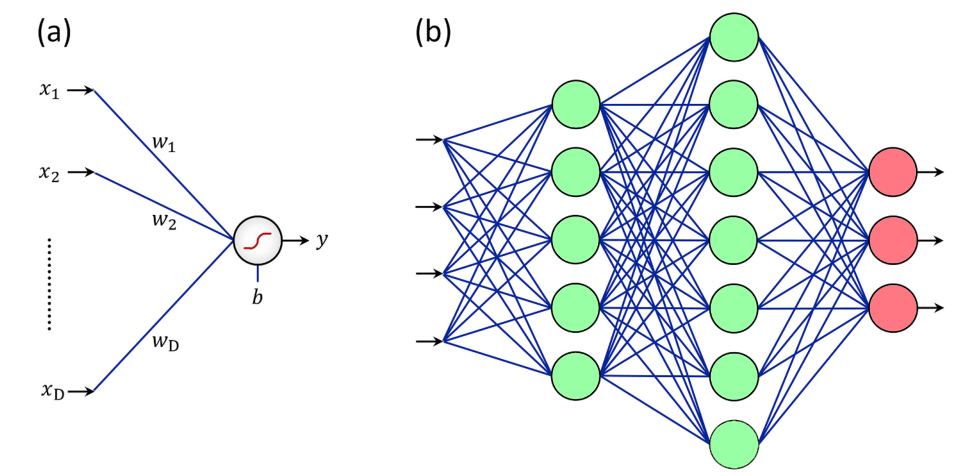
\includegraphics[scale=0.5]{figures/perceptron.png}
                \caption[The perceptron and multi-layer perceptron]{(a) A perceptron and (b) a multi-layer perceptron with four inputs in the input-layer(arrows to the left), two hidden layers(green), and three outputs in the output-layer(red).}
              	\medskip 
                \hspace*{15pt}\hbox{\scriptsize Credit: \citeauthor{razavi2021deep_exp_DL}\cite{razavi2021deep_exp_DL}}
                \label{Perceptron / MLP}
            \end{figure}
        
        The architecture of the \gls{ann} consist of an input layer, a user defined number of \textit{hidden layers} and finally an output layer. A \gls{mlp} is a type of network called \textit{feed-forward} \gls{ann} because the data flows from the input to the output layer. The parameters that are adjusted through training (explained in section XXX) are all the weights between every neuron in the network and the individual biases. The intuition for the MLP depicted in \ref{Perceptron / MLP} is that different neurons will fire with varying strengths depending on the input, resulting in different outputs.
        
    \subsection{Activation function} \label{activation function}
        The activations function is what enables the \gls{ann} to learn non-linear features \cite{razavi2021deep_exp_per}. The reason you need it is that a network consisting of only linear layers will just be the same as a single linear layer \cite{razavi2021deep_exp_per}. The activation function used in this thesis was the ReLU which stands for rectified as described in \cite{sharma2019new_activation_func}. The formula for it is as follows:
            \begin{equation} \label{relu_eq}
                f(x) = max(0,x)
            \end{equation}
        As can be seen in figure \ref{activation_fig} the function is 0 while x is less than 0 and then linear. Intuitively, this function can make a selection of neurons in figure \ref{MLP} send their computed value forth, and some  other neurons output nothing. This can result in greater efficiency and faster training, as not all neurons are active \cite{sharma2019new_activation_func}.
        
        An example of another activation function is the sigmoid \cite{sharma2019new_activation_func}, which transforms the values in the range 0 to 1. I will list the formula and have included it in the plot \ref{activation_fig}, but will not go any further as it is not necessary for understanding this thesis. Sigmoid formula:
            \begin{equation} \label{sigmoid_eq}
                f(x) = \dfrac{1}{e^{-x}} 
            \end{equation}
            
            \begin{figure}[H]
                \centering
                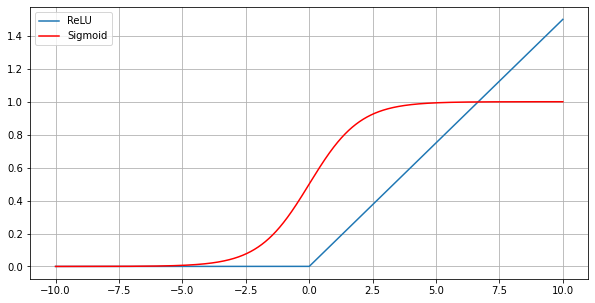
\includegraphics[scale=0.5]{figures/activation.png}
                \caption[ReLu and sigmoid]{A ReLU function (blue) and a sigmoid function (red)}.
              	\medskip 
                \label{activation_fig}
            \end{figure}

\section{Training Neural Networks} \label{training neural networks}
    \citeauthor{Goodfellow-et-al-2016_NN}\cite{Goodfellow-et-al-2016_NN} describes \gls{ann} as an unknown function \textit{\^{f}} that maps an input \textbf{x} to an output \textbf{y}. The goal is then to approximate some optimal function \textit{f} through learning from examples. In supervised tasks, the data instructs the output layer exactly how it should perform and what \textbf{y} should look like. Although, the data does not instruct the individual \textit{hidden layers} how to perform to produce this desired output. When the data flow through the network, it produces outputs \textbf{\^{y}}, this is called the \textit{forward-propagation step}. By using a \textit{loss function} comparing the true \textbf{y} values to the estimated values \textbf{\^{y}}, you get a measurement of the network's \textit{error} or also called \textit{loss}. Using this loss, you step back through the network in a process called \textit{back-propagation} and calculate a value called the \textit{gradient}. The gradient is the derivative of the loss with respect to each weight and bias\cite{rumelhart1986learning_backprop}. The gradient indicates how each weight and bias in the hidden layers should be adjusted to decrease the networks' loss. Using the gradient, an optimizing algorithm (example in section \ref{batch learning}) is applied to adjust all the individual parameters, performing \textit{gradient descent}\cite{Goodfellow-et-al-2016_gradient_descent}. In what magnitude a parameter is adjusted by the optimizing algorithm is tuned through a value called the learning rate. The precise formulation is presented later in section \ref{batch learning}.
    
    In classification tasks, the network is trained to output the probability of a class given an input. To do this, \citeauthor{zhou2019mpce_cross_entropy}\cite{zhou2019mpce_cross_entropy} describes a \textit{softmax} function that calculates the probability of each class with a sum of 1 across all classes as the last layer of a classification \gls{ann}. This probability is then the input to a loss function called \textit{cross entropy}, which calculate a loss based on probabilities in this way:
        \begin{equation} \label{cross_entropy}
            loss = - \sum^{n}_{i=1} y_{i}\log(\hat{y_{i}})
        \end{equation}
    
    where \textit{n} is the number of classes, $y_{i}$ is the true value, and $\hat{y_{i}}$ is the output from the softmax for the $i^{th}$ class. A variant of this function is called \textit{weighted} cross entropy\cite{ho2019real_weighted_cross_entropy}, and with this, you can adjust the weighting different classes have on the calculated loss. It is often used when dealing with class imbalances, and hence in this thesis.

    
    %By repeatedly applying forward-propagation, back-propagation and some optimizing algorithm on new examples as stated by \citeauthor{Goodfellow-et-al-2016_NN}, you train a network to approximate the optimal function \textit{f}.
    

\subsection{Batch learning} \label{batch learning}
        \begin{quote}
        "\textit{A recurring problem in machine learning is that large training sets are necessary for good generalization, but large training sets are also more computationally
        expensive."} - (\citeauthor{Goodfellow-et-al-2016_SGD}\citeyear{Goodfellow-et-al-2016_SGD}, page 152)
    \end{quote}
    
    The problem, described in the quote above, arises when you have a large dataset, and you would calculate the loss values of all samples before updating the parameters in your network\cite{Goodfellow-et-al-2016_SGD}. Depending on your hardware, this could lead to a crash or slow learning due to heavy memory demands. A solution is then to choose a number of uniformly chosen examples from the entire dataset forming a \textit{minibatch}, with the intent to approximately estimate the true gradient using this smaller fraction of the dataset. Then you would update the parameters of your network based on this and repeat on a new batch. When you have run this process on all your data, you say that an \textit{epoch} has passed. The size of this minibatch can vary from one example, to hundreds and the size chosen can heavily affect training and is very reliant on a fitting learning rate\cite{wilson2001need_learning_rate}. A widely used optimization algorithm is \textit{\gls{sgd}}\cite{Goodfellow-et-al-2016_SGD}, which utilizes this minibatch form of training. \gls{sgd} is the algorithm used in this thesis. In the more precise from batch learning is formulated as:
    
        \begin{equation} \label{batch_learning_eq}
            \Theta = \arg \min_{\Theta}\dfrac{1}{N} \sum^{N}_{i=1} loss (x_{i},\Theta)
        \end{equation}
    
    where \gls{sgd} optimize the parameters $\Theta$ of the network, $x_{1..N}$ is the training data, and $x_{1..m}$ is a minibatch of the training data.

\subsection{Momentum}


\subsection{Regularization}
    Regularization as described by \citeauthor{kukavcka2017_regularization}\cite{kukavcka2017_regularization} is a small alternation or technique added to the training process that has as goal to make the model generalize better on the validation and test data. This can be applied in different ways, and two used in this thesis will be described here; \textit{batch normalization} and \textit{data-augmentation}.
    
\subsubsection{Batch-Norm}
    Batch normalization is a technique applied to reduce what is called \textit{internal  covariate shift}\cite{pmlr-v37-ioffe15_batch_norm}. This is defined as the change in the distribution of activations in \gls{ann}s hidden layers caused by the change in the networks parameters when training. As the hidden layers depend on the activations of all layers before them, this has been shown to slow down and destabilize the training process. The solution to this problem is the implementation of \textit{batch normalization}. By using the activations from all the neurons in a hidden layer, a \textit{mean} and \textit{variance} is calculated, and is done per batch. These values are then used to normalize the activations of the hidden layer, and each hidden layer are given two additional learnable parameters $\gamma$ and $\beta$, that perform a linear transformation of the normalized activations, defined as such:
    
        \begin{equation} \label{batch_normalization}
            \textrm{Batch normalized activations} =   \gamma Z^{(i)}_{norm} + \beta
        \end{equation}
    
    where $Z^{(i)}_{norm}$ is the normalized activations for the $i^{th}$ hidden layer. The learnable parameters make the \gls{ann} able to adjust and shift the distribution through the training process. The result is a faster and more stable training process. 

\subsubsection{Data-Augmentation}
    The previous regularization method is applied during training, but \textit{data-augmentation} is applied to the data itself\cite{kukavcka2017_regularization}. There are several methods available, but the two used in this work are: \textit{adding noise} and \textit{vertical flipping}. One example of applying noise is to add Gaussian values with a mean of 0 and some user-defined variance to each pixel. This adds more randomness to the data, making the model learn more general features instead of specific, hence increasing generalization performance. Other methods of applying noise are described in \citeauthor{kukavcka2017_regularization}\cite{kukavcka2017_regularization}. \todo{mer detalj} The \textit{vertical flipping} is a simple yet effective transformation where you flip the input along a certain axis. Vertical flipping is justified in this case, as this never change where the seafloor and surface is in an echogram. Both methods make the model generalize better by producing new unseen samples by changing the way the data is represented.  An example of each method can be seen in figure \ref{data augmentation fig}:
    
    \begin{figure}[H]
        \centering
        
        \subfloat[Gaussian noise added to each pixel.]{
        	\includesvg[inkscapelatex=false,width=0.9\textwidth,keepaspectratio]{figures/add_noise.svg}}
        	%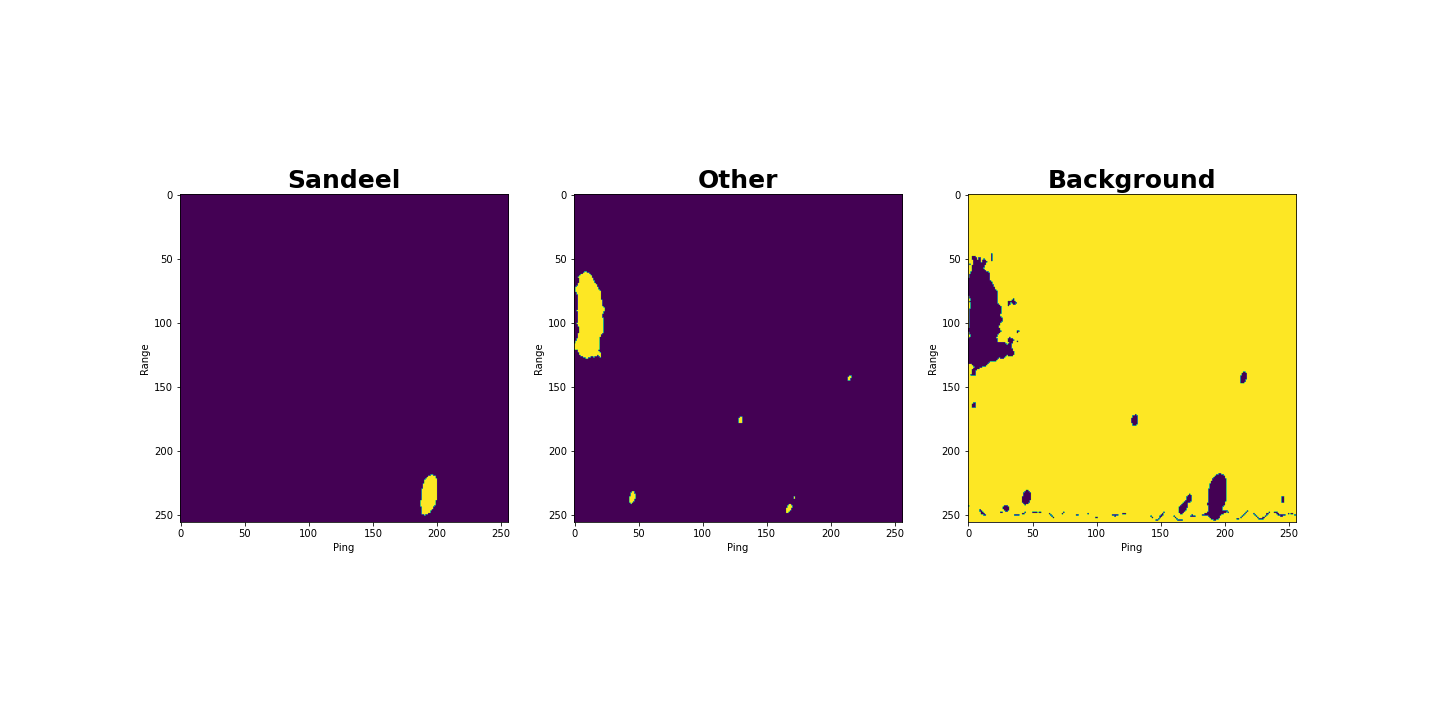
\includegraphics[width=1\textwidth]{figures/data_sample.png} } 
        
        \subfloat[Vertical flipping.]{
        	\includesvg[inkscapelatex=false,width=0.9\textwidth,keepaspectratio]{figures/vertical_flip.svg}}
        
        
        \caption[Two data augmentation examples]{Two augmentation methods applied to the same image.}
        \label{data augmentation fig}
        
        \end{figure}
    
    
\clearpage
\section{Computer vision} \label{computer vision}
    \textbf{Computer vision} is a very popular field of research within deep learning\cite{voulodimos2018deep_computer_vision}. This is because it has mainly focused around tasks we humans do naturally, while computers would struggle. Examples are facial recognition, object detection and many more. Some work also went beyond human capability, like \citeauthor{davis2014visual_deep_video_audio}s\cite{davis2014visual_deep_video_audio} work, where he recovered sounds from the vibrations they induced in objects captured on video. There are many methods in the field of computer vision, but I will focus on the \gls{cnn}.
    
    
    
\subsection{Convolutional neural network} \label{cnn}
    The \textbf{\gls{cnn}} are a type of \gls{ann}s that are primarily used in machine learning tasks concerning images\cite{o2015introduction_convolutions}.The need for the convolutional operation stemmed from the fact that images input to a regular \gls{ann} produces a large amount of learnable parameters. An example 512×512 low-resolution image with a first layer of 1 neuron would have $1*512*512 = 262144$ weights alone.  To solve this issue and have fewer learnable parameters, the \gls{cnn} is built around 3 main components\cite{o2015introduction_convolutions}; \textit{convolutional layer}, \textit{pooling layer} and a \textit{fully-connected layer}. An example \gls{cnn} is illustrated in figure \ref{convolutional_neural_network_fig} and each main component will be explained later in this section.

    \begin{figure}[H]
        \centering
        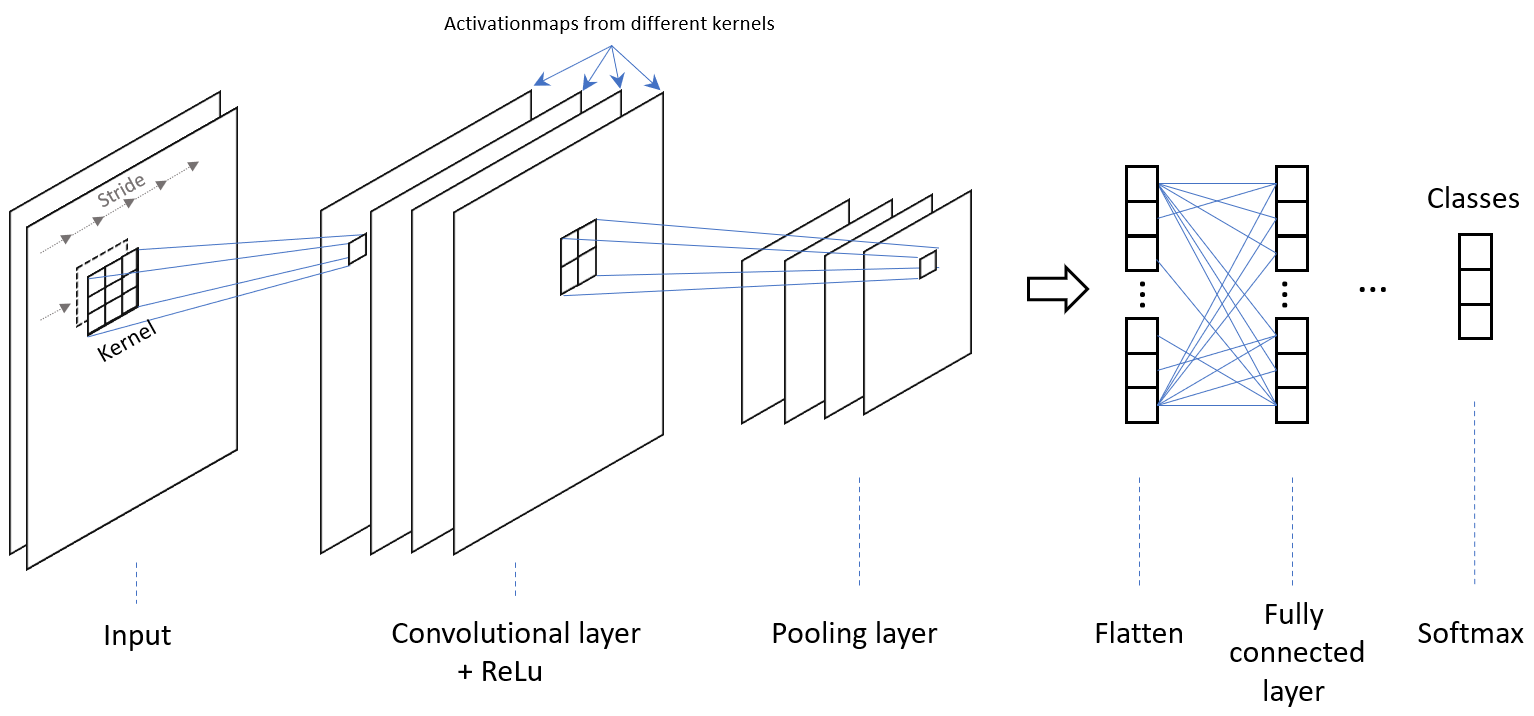
\includegraphics[scale=0.4]{figures/conv_net.png}
        \caption[Convolutional neural network example]{Illustrations of the main components in a \gls{cnn}. The \textit{flatten} operation is applied here to make the output from the pooling layer compatible with the fully connected layer of regular neurons. The \textit{softmax} is an example final layer.}
      	\medskip 
        \label{convolutional_neural_network_fig}
    \end{figure}
    
    \subsubsection{Convolutional layer}
     \citeauthor{o2015introduction_convolutions}\cite{o2015introduction_convolutions} describes that the convolutional layer consists of a number of learnable  weight matrices each consisting of three dimensions; \textit{height}, \textit{width} and \textit{depth} written as: \textit{height} x \textit{width} x \textit{depth}. From now, this matrix will be called the kernel. The height and the width of the kernel are parameters defined by the user and are usually small, but the depth will always equal the number of channels in the input. This results in kernels being written only as: \textit{height} x \textit{width}. The kernel slides over the input, and is applied to different locations of the input, also called the current \textit{receptive field}. When applied, a single scalar value is computed that is the weighted sum of the kernels weights and the corresponding values in the receptive field. This scalar value is called the \textit{activation}, and is often fed through non-linear activation function like ReLu. The sliding operation is constructed around a value called \textit{stride} and is the amount of horizontal positions to move the kernel between each calculation. If it is not possible to move in the horizontal direction, the kernel will move rows down vertically equal to the stride and begin anew. After sliding over the entire input, a complete 2D activation map has been created, one such map for each kernel. The idea is that each of these kernels will learn to identify different features in the input, and an example of a horizontal edge detector can be seen in figure \ref{convolutional_fig}.
    \clearpage
    \begin{figure}[H]
        \centering
        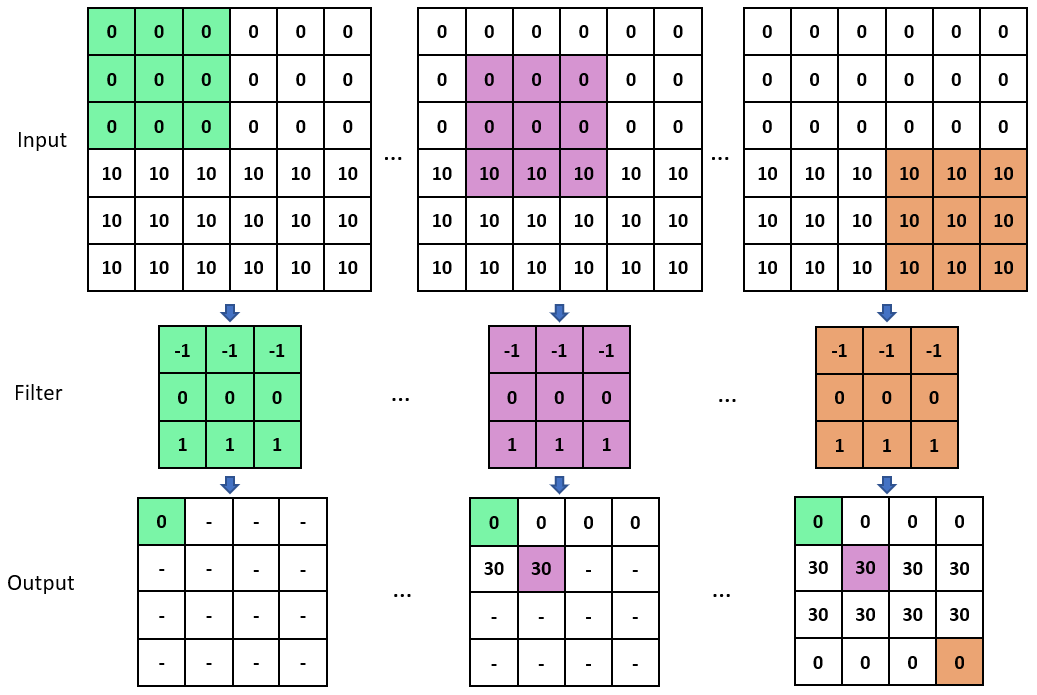
\includegraphics[scale=0.4]{figures/convolutions.png}
        \caption[Horizontal edge detector example]{Illustration of a \textit{valid} convolutional operation. The kernel is applied repeatedly across the input. The size of input is 6x6, kernel size is 3x3 and stride 1, resulting in overlapping operations and output size being 4x4. The figures to the right show the input, kernel and output(activation) as color gradings, where the color gets darker if the values are low. This example is a horizontal edge detector, and the result is large values in the activation map along the border between the values of 0 and 10 in the input, which could have been colors in a picture.}
      	\medskip 
        \label{convolutional_fig}
    \end{figure}
    
    The receptive field will start as small regions, but as you apply more convolutional layers, the receptive field will have access to increasing context\cite{o2015introduction_convolutions}. This is illustrated in figure \ref{receptive_field_fig}, and kernels in early layers learn to identify simple features while later combine these to identify complex features. In the same figure, this could for example have been the upper and lower jaw of the leftmost cat being combined to recognize a mouth in later layers. The kernel is slid over its entire input and so utilizes what is called \textit{parameter sharing }, as the same weights are used repeatedly across the previous the input. Another positive consequence is that the location of the feature in the input is not relevant to a convolutional neural network. Combined, this creates a layer able to detect features in an input with fewer learnable parameters than a normal \gls{ann}. 
    
    \begin{figure}[H]
        \centering
        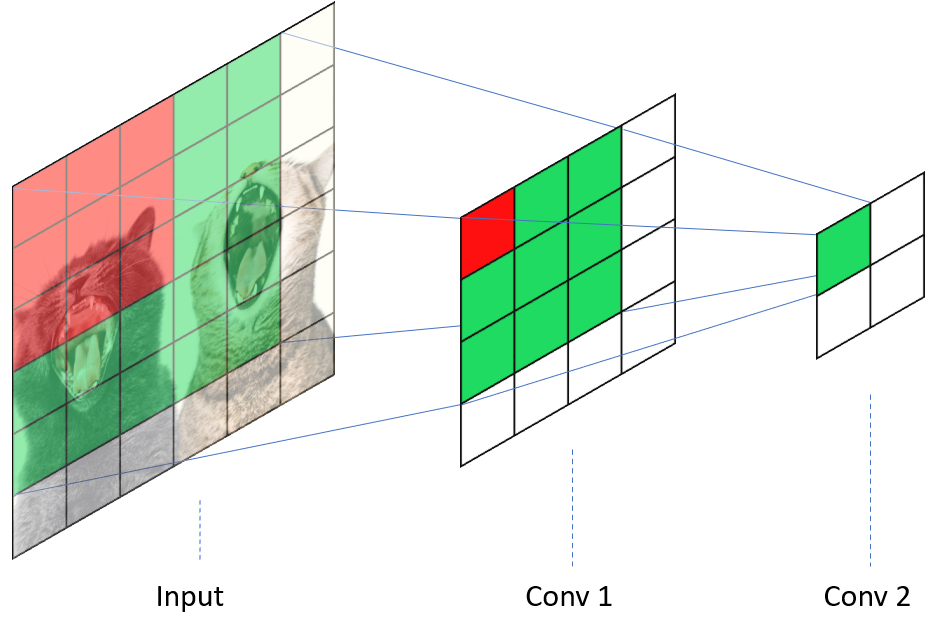
\includegraphics[scale=0.4]{figures/receptive_field.png}
        \caption[Receptive field]{The activation maps from two convolutional layers with 3×3 kernels and stride 1. The first convolutions receptive field is marked as red. On its activation map, a new convolutional layer is applied. Its first receptive field is outlined in green, which translates to a large area in the input.}
      	\medskip 
        \label{receptive_field_fig}
    \end{figure}

    %The complete \textit{convolutional operation} performed by a convolutional layer consists of applying this kernel to the entire input. Producing activations for different regions of the input. This reduces the dimension of the input to a 2D activation output, but you may apply several kernels to increase the channels, as each will create a new 2D channel in the activations. A convolutional operation is often followed up with an element wise nonlinear activation function to its activations, like a ReLu. The kernels will through training learn to detect different features in the input, and so in a \gls{cnn} the first layers will often detect simple features like edges. Later layers will then detect more complex features like cars and houses, combining the activations from different earlier layers. The last layer consists of a \textit{fully connected} layer of regular neurons to determine the output, but implementations of networks with only convolutional operations exists like U-Net which will be described\cite{unet_ronneberger2015} in section \ref{unet} utilizing 1x1 convolutions. A more detailed example can be found in figure \ref{convolutional_fig} which looks at how a convolution with a horizontal edge detecting kernel is applied to a single channel or an equivalent 2D input. 
    
    Reductions in the spatial size\cite{o2015introduction_convolutions} will normally occur with the standard convolutions, and this type is called \textit{valid convolutions}. By applying a padding with zeros around the input, you can retain the dimensions of the input. The effect is that more convolutional operations fits in the new padded input, hence larger output size. This is called a \textit{same convolution}. Illustrated in figure \ref{same_convolutional_fig}.
    
    \begin{figure}[H]
        \centering
        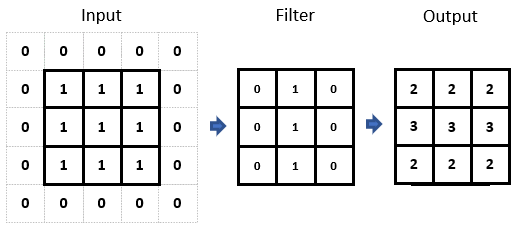
\includegraphics[scale=0.6]{figures/same_convolutions.png}
        \caption[Same convolution example]{Illustration of a \textit{same} convolutional operation. The size of the input is 3×3, but after padding with zeros the size is 5×5, kernel size is 3×3 and stride is 1. Resulting in an activation map if size 3×3, hence conserving the input size.}
      	\medskip 
        \label{same_convolutional_fig}
    \end{figure}
    
    
    
\subsubsection{Pooling layer}
    There are many different kinds of pooling layers, but I will focus on the variant called max pool. The \textbf{max pool layer} reduces the \textit{height} and \textit{widht} of its input\cite{o2015introduction_convolutions}. Like a convolutional operation, the max pool looks at a region of the input, but then instead applies a \textit{max} operation. The kernel size is given in \textit{height} x \textit{width}, and is applied individually to each dimension of the input. This reduces the height and width, but not the channels. The most common setting is 2×2 with a stride 2, which results in decreasing the size to 25\%. On it own, the max pool have no learnable parameters and is applied to decrease the computation complexity of the \gls{cnn}.

    \begin{figure}[H]
        \centering
        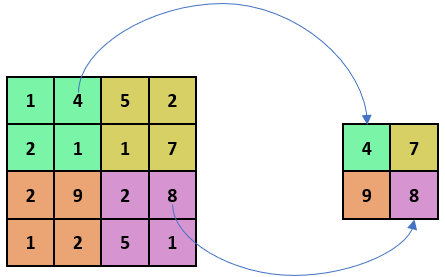
\includegraphics[scale=0.5]{figures/max_pool.png}
        \caption[The max pool operation]{Illustration of the max pool operation with size 2×2 and stride 2.}
      	\medskip 
        \label{maxpool_fig}
    \end{figure}

\subsubsection{Fully connected layer}
    \begin{figure}[H]
        \centering
        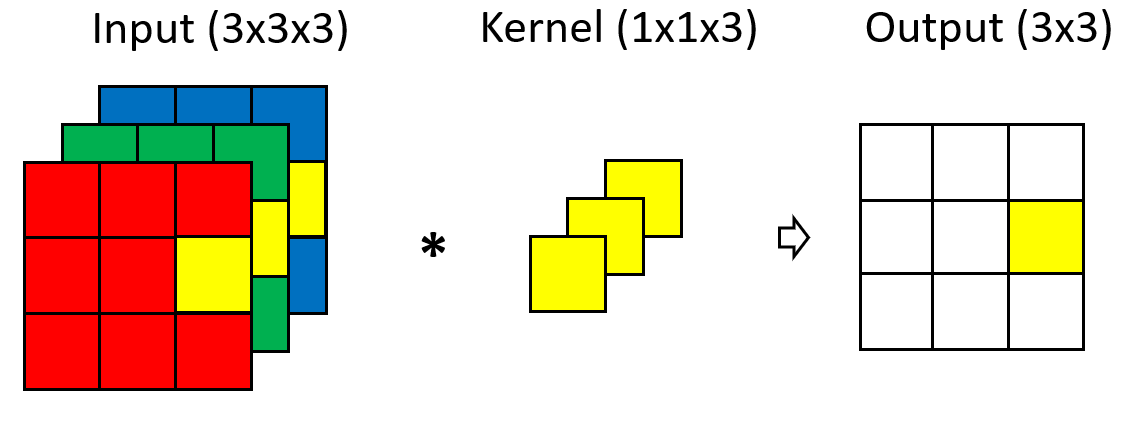
\includegraphics[scale=0.35]{figures/1x1.png}
        %\includesvg[inkscapelatex=false,scale=0.3,keepaspectratio]{figures/Bilde1.svg}
        \caption[1x1 convolution]{Illustration of the 1x1 convolution with stride 1.}
      	\medskip 
        \label{1x1_fig}
    \end{figure}
    \citeauthor{lin2013network_in_network_1x1}\cite{lin2013network_in_network_1x1} proposed the convolutional layer with kernel size 1×1 and stride 1, followed by a activation function, as an equivalent to the regular hidden layer shown earlier in figure \ref{Perceptron / MLP}\cite{lin2013network_in_network_1x1}. The 1x1 layer will take the weighted sum along a 1x1 slice through all channels of the input, as illustrated in figure \ref{1x1_fig}. This is the exact same as applying a fully connected layer to the same values. As this preserves \textit{height} and \textit{width}, this can then be used as a tool for alterations of the depth of a network by specifying the desired number of kernels. In this work, it is used mainly to map high dimensional feature maps to the desired number of classes. In figure \ref{convolutional_neural_network_fig} with the example \gls{cnn}, a normal fully connected layer of neurons has been used, but could have been replaced with 1×1 convolution. Thus creating a network with only convolutional layers. 
    
    

\subsubsection{Transposed convolutions}
    A transposed convolution is an operation performing the opposite operation compared to a regular convolution\cite{dumoulin2016guide_transposed_convolution}. This means taking an input and with a similar \textit{kernel} as described earlier in \ref{cnn} and now instead map this to a higher spatial size. In example figure \ref{transposed_conv_fig} a 2D 2×2 input is fed to a transposed convolutional layer with kernel size 2×2. The whole kernel is multiplied element wise to the input and proceeds to produce values in a temporary matrix initialized with zeros(empty cells in the figure). The calculated values in the temporary matrix are situated correctly relative to the input. These temporary matrices are then summed over, producing the output. This operation is repeated for all channels, retaining the depth of the input. 
    
    \begin{figure}[H]
        \centering
        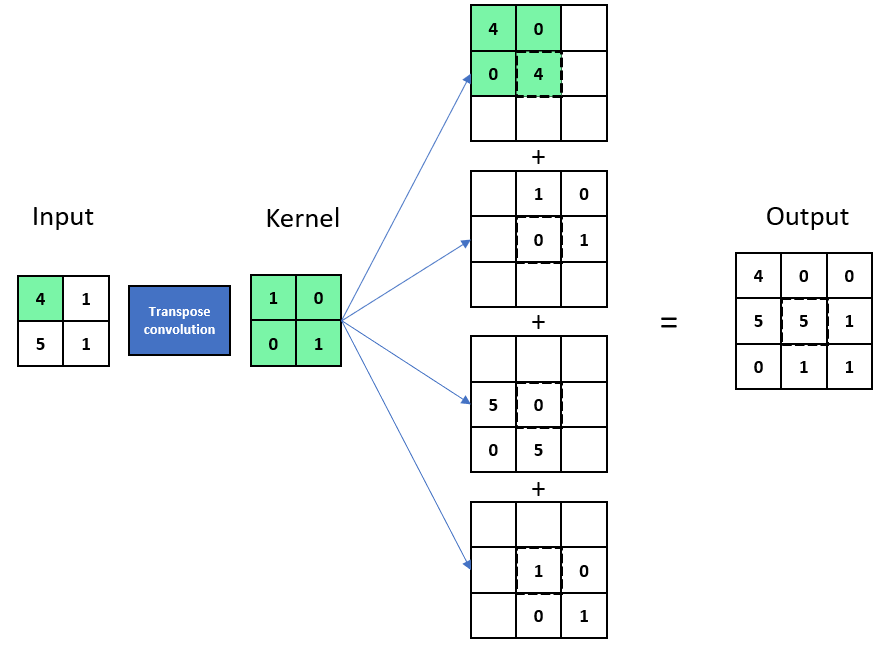
\includegraphics[scale=0.5]{figures/transpose_convolution.png}
        \caption[Transposed convolution]{Illustration of the transposed convolution operation with kernel size 2×2 and stride 1. The green color shows one of the intermediate computations. The center value of each crop is outlined to illustrate the summation step as these overlaps.}
      	\medskip 
        \label{transposed_conv_fig}
    \end{figure}
    
\subsubsection{Segmentation}
    Segmentation is a computer vision task where the objective is to assign one or several classification masks to the input\cite{He_2017_ICCV_segmentation}. This is again split into two different categories; \textit{semantic} and \textit{instance} segmentation. In semantic segmentation, you assign each pixel in the input to predefined classes. While in instance segmentation, you increase the complexity by applying semantic segmentation and in parallel assigning a bounding box to each individual object. Semantic segmentation is the variant used in this thesis, and examples of both can be viewed in figure \ref{segmentation_fig}.
    
    \begin{figure}[H]
        \centering
        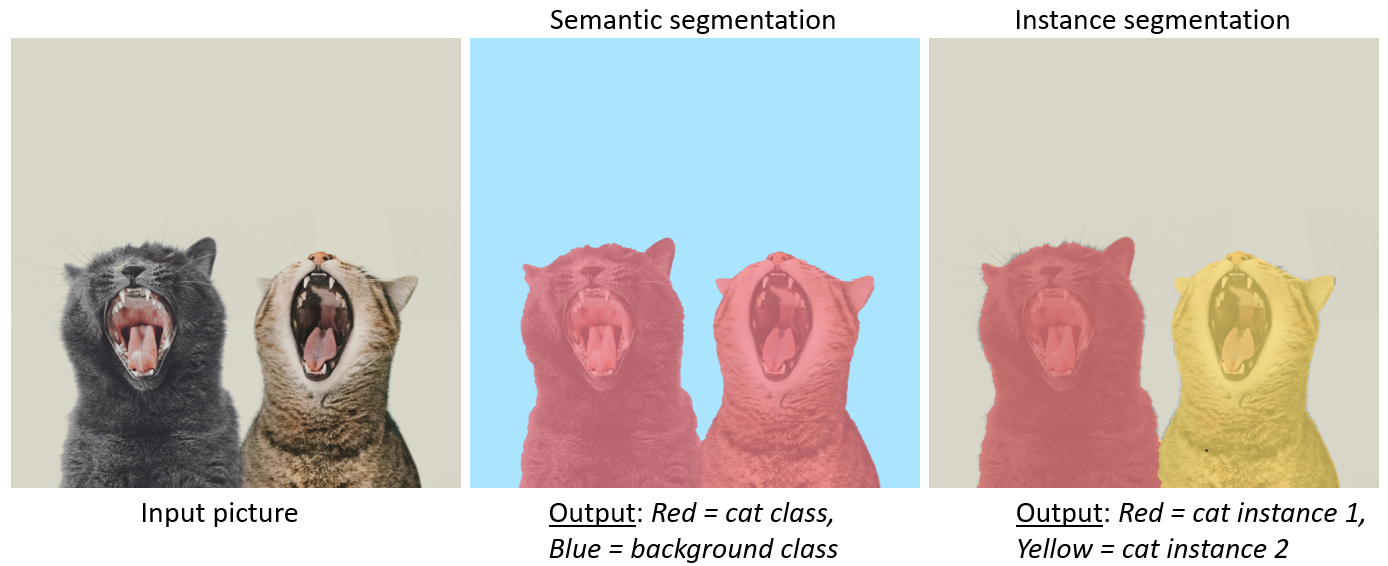
\includegraphics[scale=0.4]{figures/segmentation.png}
        \caption[Difference between semantic and instance segmentation]{Illustration of the difference between semantic and instance segmentation.}
      	\medskip 
        \label{segmentation_fig}
    \end{figure}
    
    

\subsection{U-Net} \label{unet}
    In this part, I introduce the architecture of the deep learning \gls{ann} used in this thesis, called U-Net. This is a fully convolutional state-of-the-art\cite{rajak2021segmentation} semantic segmentation \gls{ann} and was initially developed for biomedical use by \citeauthor{unet_ronneberger2015}\cite{unet_ronneberger2015}. The \gls{crimac} used this model in their project (described in \ref{unet_paper_acoustic}) and had to do some small modifications to the network to fit their task. This modified U-Net is the one presented in this section, as this is the one used in the experiments. The core functionality of the network stays true to the original Unet, and the alterations done to the original will be explained later in this section.
    
    \begin{figure}[H]
        \centering
        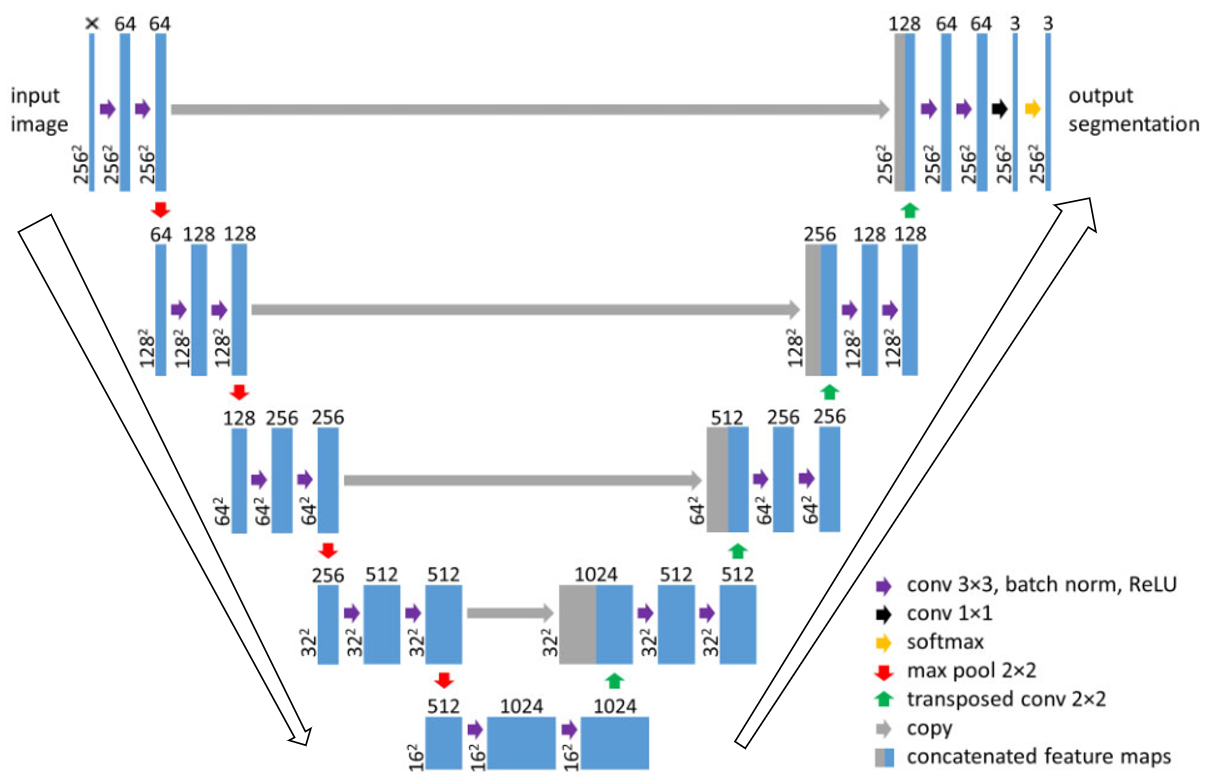
\includegraphics[scale=0.5]{figures/unet_arrows.png}
        \caption[U-Net architecture]{U-Net architecture, the downwards facing arrow illustrates the contracting path and the one facing upwards is the expanding path.}
      	\medskip 
        \label{unet_fig}
        \hspace*{15pt}\hbox{\scriptsize Credit: \citeauthor{brautaset2020acoustic}\cite{brautaset2020acoustic}}
    \end{figure}
    
    Unet utilized what \citeauthor{unet_ronneberger2015}\cite{unet_ronneberger2015} called a contracting path to identify what was in a picture, while an expanding path to localize where it was. These two branches were symmetrical, and together they formed a U-shape, giving the network its name. The contracting path can be looked at as five different stages of processing, from top to bottom, in figure \ref{unet_fig}. Each stage applied the same operations to its given input. For each stage, this consisted first of two 3x3 same convolutions with their individual ReLu activation functions. Initially, the feature channels would be increased to 64, and later doubled for each contracting stage. The convolutions were followed by a 2×2 max pooling operation with stride 2 to decrease the resolution of the output from the convolutional operations, and then send this feature map down to the next stage. At the bottom stage, the only things that changed was the use of transpose convolutions instead of max pooling to now increase the resolution. At each subsequent stage going back up the expanding path, the number of feature channels were halved. To aid the localization, the output of the previous stage would be concatenated with the output feature map of a stage from the contracting path with the same size. At the last stage, when the resolution had reached it original size, a 1×1 convolution was applied instead of increasing the resolution. The 1×1 convolution mapped the 64 feature channels to the 3 classes. The softmax was then calculated between these classes, giving each pixel a value between [0,1], summarized over all classes to 1. Hence, giving you a segmentation map of each class with the same size as the input. 
    
    %In this thesis, this will be a semantic segmentation of the classes \textit{background}, \textit{other } and most importantly \textit{sandeel}.
    
    Minor changes were made to adapt\citeauthor{unet_ronneberger2015}s original U-Net to the acoustic data used in \ref{unet_paper_acoustic}, as the input now had the form 4 x 256 x 256. The four channels being the frequencies used. The convolutions were set to \textit{same} instead of \textit{valid}, as were the original setting. This was done to make the size of the input and output match. Further, batch normalization was added to each convolution. 
    


        

    
    